\let\negmedspace\undefined
\let\negthickspace\undefined
%\RequirePackage{amsmath}
\documentclass[journal,12pt,twocolumn]{IEEEtran}
\usepackage{gensymb}
\usepackage{polynom}
\usepackage{amssymb}
\usepackage[cmex10]{amsmath}
\usepackage{amsthm}
\usepackage{stfloats}
\usepackage{bm}
\usepackage{enumitem}
\usepackage{mathtools}
  %\usepackage{tikz}
% \usepackage{circuitikz}
% \usepackage{verbatim}
%\usepackage{tfrupee}
  %\usepackage[breaklinks=true]{hyperref}
%\usepackage{stmaryrd}
%\usepackage{tkz-euclide} % loads  TikZ and tkz-base
%\usetkzobj{all}
\usepackage{listings}
    \usepackage{color}                                            
    \usepackage{array}                                            
    \usepackage{longtable}                                        
    \usepackage{calc}                                             
    \usepackage{multirow}                                         
    \usepackage{hhline}                                           
    \usepackage{ifthen}                                           
  %optionally (for landscape tables embedded in another document): 
    \usepackage{lscape}     
% \usepackage{multicol}
% \usepackage{chngcntr}
%\usepackage{enumerate}
%\usepackage{wasysym}
%\newcounter{MYtempeqncnt}
\DeclareMathOperator*{\Res}{Res}
\DeclareMathOperator*{\equals}{=}
%\renewcommand{\baselinestretch}{2}
\renewcommand\thesection{\arabic{section}}
\renewcommand\thesubsection{\thesection.\arabic{subsection}}
\renewcommand\thesubsubsection{\thesubsection.\arabic{subsubsection}}
\renewcommand\thesectiondis{\arabic{section}}
\renewcommand\thesubsectiondis{\thesectiondis.\arabic{subsection}}
\renewcommand\thesubsubsectiondis{\thesubsectiondis.\arabic{subsubsection}}
% correct bad hyphenation here
\hyphenation{op-tical net-works semi-conduc-tor}
\def\inputGnumericTable{}                                 
\lstset{
%language=C,
frame=single, 
breaklines=true,
columns=fullflexible
}
%
\begin{document}
%
\newtheorem{theorem}{Theorem}[section]
\newtheorem{problem}{Problem}
\newtheorem{proposition}{Proposition}[section]
\newtheorem{lemma}{Lemma}[section]
\newtheorem{corollary}[theorem]{Corollary}
\newtheorem{example}{Example}[section]
\newtheorem{definition}[problem]{Definition}
%\newtheorem{thm}{Theorem}[section] 
%\newtheorem{defn}[thm]{Definition}
%\newtheorem{algorithm}{Algorithm}[section]
%\newtheorem{cor}{Corollary}
\newcommand{\BEQA}{\begin{eqnarray}}
\newcommand{\EEQA}{\end{eqnarray}}
\newcommand{\define}{\stackrel{\triangle}{=}}
\newcommand*\circled[1]{\tikz[baseline=(char.base)]{
    \node[shape=circle,draw,inner sep=2pt] (char) {#1};}}
\bibliographystyle{IEEEtran}
%\bibliographystyle{ieeetr}
%
\providecommand{\mbf}{\mathbf}
\providecommand{\pr}[1]{\ensuremath{\Pr\left(#1\right)}}
\providecommand{\qfunc}[1]{\ensuremath{Q\left(#1\right)}}
\providecommand{\sbrak}[1]{\ensuremath{{}\left[#1\right]}}      % []
\providecommand{\lsbrak}[1]{\ensuremath{{}\left[#1\right.}}
\providecommand{\rsbrak}[1]{\ensuremath{{}\left.#1\right]}}
\providecommand{\brak}[1]{\ensuremath{\left(#1\right)}}         % ()
\providecommand{\lbrak}[1]{\ensuremath{\left(#1\right.}}
\providecommand{\rbrak}[1]{\ensuremath{\left.#1\right)}}
\providecommand{\cbrak}[1]{\ensuremath{\left\{#1\right\}}}      % {}
\providecommand{\lcbrak}[1]{\ensuremath{\left\{#1\right.}}
\providecommand{\rcbrak}[1]{\ensuremath{\left.#1\right\}}}
\theoremstyle{remark}
\newtheorem{rem}{Remark}
\newcommand{\sgn}{\mathop{\mathrm{sgn}}}
\providecommand{\abs}[1]{\ensuremath{\left\vert#1\right\vert}}
\providecommand{\res}[1]{\Res\displaylimits_{#1}} 
\providecommand{\norm}[1]{\ensuremath{\left\lVert#1\right\rVert}}
%\providecommand{\norm}[1]{\lVert#1\rVert}
\providecommand{\mtx}[1]{\mathbf{#1}}
\providecommand{\mean}[1]{\ensuremath{E\left[ #1 \right]}}
\providecommand{\fourier}{\overset{\mathcal{F}}{ \rightleftharpoons}}
%\providecommand{\hilbert}{\overset{\mathcal{H}}{ \rightleftharpoons}}
\providecommand{\system}{\overset{\mathcal{H}}{ \longleftrightarrow}}
	%\newcommand{\solution}[2]{\textbf{Solution:}{#1}}
\newcommand{\solution}{\noindent \textbf{Solution: }}
\newcommand{\cosec}{\,\text{cosec}\,}
\providecommand{\dec}[2]{\ensuremath{\overset{#1}{\underset{#2}{\gtrless}}}}
\newcommand{\myvec}[1]{\ensuremath{\begin{pmatrix}#1\end{pmatrix}}}
\newcommand{\mydet}[1]{\ensuremath{\begin{vmatrix}#1\end{vmatrix}}}
\newcommand*{\permcomb}[4][0mu]{{{}^{#3}\mkern#1#2_{#4}}}
\newcommand*{\perm}[1][-3mu]{\permcomb[#1]{P}}
\newcommand*{\comb}[1][-1mu]{\permcomb[#1]{C}}
%
%used because document has section:
\numberwithin{equation}{section}
\numberwithin{figure}{section}
\numberwithin{table}{section}
\numberwithin{equation}{section}
\numberwithin{problem}{section}
%\numberwithin{definition}{section}
\makeatletter
\@addtoreset{figure}{problem}
\makeatother

\let\StandardTheFigure\thefigure
\let\vec\mathbf
%\renewcommand{\thefigure}{\theproblem.\arabic{figure}}
    %\renewcommand{\thefigure}{\theproblem}
%\setlist[enumerate,1]{before=\renewcommand\theequation{\theenumi.\arabic{equation}}
%\counterwithin{equation}{enumi}
%\renewcommand{\theequation}{\arabic{subsection}.\arabic{equation}}

\def\putbox#1#2#3{\makebox[0in][l]{\makebox[#1][l]{}\raisebox{\baselineskip}[0in][0in]{\raisebox{#2}[0in][0in]{#3}}}}
     \def\rightbox#1{\makebox[0in][r]{#1}}
     \def\centbox#1{\makebox[0in]{#1}}
     \def\topbox#1{\raisebox{-\baselineskip}[0in][0in]{#1}}
     \def\midbox#1{\raisebox{-0.5\baselineskip}[0in][0in]{#1}}
\vspace{3cm}

\title{Random Variable Generation, AI1110}
\author{Rajiv Shailesh Chitale (cs21btech11051)}	

\maketitle
\tableofcontents
\bigskip
\renewcommand{\thefigure}{\theenumi}
\renewcommand{\thetable}{\theenumi}


\begin{abstract}
This manual provides solutions to simple examples of generation of random numbers
\end{abstract}
%%
\section{Uniform Random Numbers}
Let $U$ be a uniform random variable between 0 and 1.
\begin{enumerate}[label=\thesection.\arabic*
,ref=\thesection.\theenumi]
\item Generate $10^6$ samples of $U$ using a C program and save into a file called uni.dat .
\\
\solution Download the following c code. Run it to generate samples of $U$.
\begin{lstlisting}
wget https://github.com/cs21btech11051Rajiv/AI1110_assignments/blob/main/manual1/q1/1p1.c
\end{lstlisting}
%
\item
Load the uni.dat file into python and plot the empirical CDF of $U$ using the samples in uni.dat. The CDF is defined as
\begin{align}
    F_{U}\brak{x} = \pr{U \le x}
\end{align}
\\
\solution The empirical CDF of U is plotted in \ref{fig:uni_cdf}
using the code below
\begin{lstlisting}
wget https://github.com/cs21btech11051Rajiv/AI1110_assignments/blob/main/manual1/q1/1p2.py
\end{lstlisting}
\begin{figure}[ht!]
    \centering
    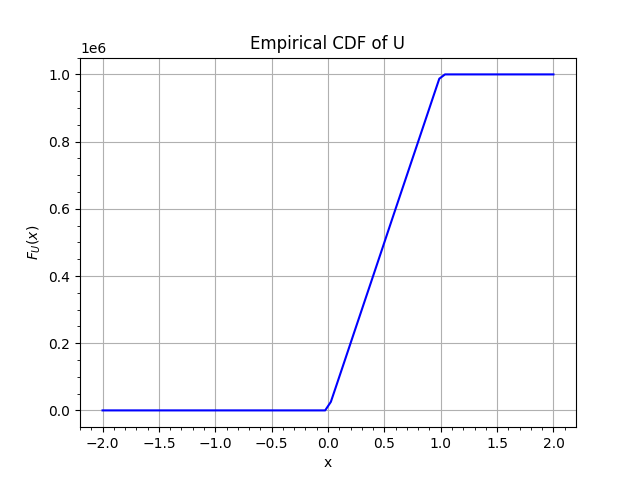
\includegraphics[width=\columnwidth]{./figs/fig1.2.png}
    \caption{The CDF of $U$}
    \label{fig:uni_cdf}
\end{figure}
%
\item
Find a theoretical expression for $F_{U}\brak{x}$.
\\
\solution The PDF has a uniform distribution,
\begin{align}
    p_U\brak{x} &=
        \begin{cases}\frac{1}{1-0} & 0 \le x \le 1 \\
        0 & otherwise
    \end{cases}\\
    F_{U}\brak{x} &= \int^{x}_{\infty} p_U\brak{x} dx \\
    F_U\brak{x} &=
    \begin{cases}  
        0 & x < 0\\
        \int^{x}_{0} 1 dx & 0 \le x \le 1 \\
        \int^{1}_{0} 1 dx & 1 < x
    \end{cases}\\
    F_U\brak{x} &=
    \begin{cases}  
        0 & x < 0\\
        x & 0 \le x \le 1 \\
        1 & 1 < x
    \end{cases}
    \label{eq:F_U}
\end{align}
\solution  The theoretical CDF of U is plotted in \ref{fig:theory_uni_cdf} using the code below
\begin{lstlisting}
wget https://github.com/cs21btech11051Rajiv/AI1110_assignments/blob/main/manual1/q1/1p3.py
\end{lstlisting}
\begin{figure}[ht!]
    \centering
    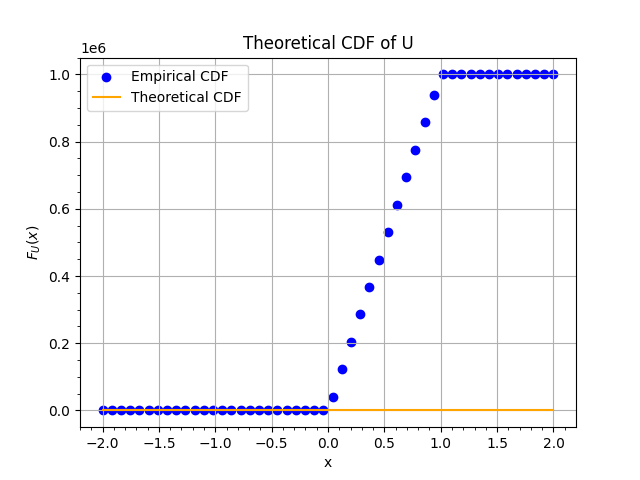
\includegraphics[width=\columnwidth]{./figs/fig1.3.png}
    \caption{The CDF of $U$}
    \label{fig:theory_uni_cdf}
\end{figure}
%
\item
The mean of $U$ is defined as
%
\begin{equation}
E\sbrak{U} = \frac{1}{N}\sum_{i=1}^{N}U_i
\end{equation}
%
and its variance as
%
\begin{equation}
    \text{var}\sbrak{U} = E\sbrak{\brak{U- E\sbrak{U}}^2} \end{equation}
Write a C program to  find the mean and variance of $U$. 
\\
\solution Run the following C file
\begin{lstlisting}
wget https://github.com/cs21btech11051Rajiv/AI1110_assignments/blob/main/manual1/q1/1p4.c
\end{lstlisting}
Results were,
\begin{align}
E\sbrak{U} = 0.500007 \\
\text{var}\sbrak{U} = 0.083301 
\end{align}
%
\item Verify your result theoretically given that
\end{enumerate}
%
\begin{align}
    E\sbrak{U^k} = \int_{-\infty}^{\infty}x^kdF_{U}\brak{x}
    \label{eq:expectation}
\end{align}
\solution Taking k as 1,
\begin{align}
    E\sbrak{U} = \int_{-\infty}^{\infty}xdF_{U}\brak{x}
\end{align}
Using expression \eqref{eq:F_U}, this simplifies to
\begin{align}
    E\sbrak{U} &= \int_{0}^{1}xdx \\
    E\sbrak{U} &= \frac{x^2}{2} \Big|_0^1 \\
    E\sbrak{U} &= 0.5
\end{align}
To calculate variance we take k=2
\begin{align}
    \text{var}\sbrak{U} &= E\sbrak{\brak{U- E\sbrak{U}}^2} \\
    \text{var}\sbrak{U} &= E\sbrak{\brak{U-0.5}^2} \\
    \text{var}\sbrak{U} &= E\sbrak{U^2 - U + 0.25}  \\
    \text{var}\sbrak{U} &= E\sbrak{U^2} - E\sbrak{U} + E\sbrak{0.25}  \\
    \text{var}\sbrak{U} &= \int_{-\infty}^{\infty}x^2dF_{U}\brak{x} - 0.5 + 0.25  \\
    \text{var}\sbrak{U} &= \int_{0}^{1}x^2dx - \frac{1}{4}  \\   
     \text{var}\sbrak{U} &= \frac{x^3}{3} \Big|_0^1 - \frac{1}{4}  \\    
     \text{var}\sbrak{U} &= \frac{1}{12} = 0.0833 \\    
\end{align}
%
\section{Central Limit Theorem}
%
\begin{enumerate}[label=\thesection.\arabic*
,ref=\thesection.\theenumi]
%
\item
Generate $10^6$ samples of the random variable
%
\begin{equation}
X = \sum_{i=1}^{12}U_i -6
\end{equation}
%
using a C program, where $U_i, i = 1,2,\dots, 12$ are  a set of independent uniform random variables between 0 and 1
and save in a file called gau.dat
\\
\solution Download the following c code. Run it to generate samples of $X$.
\begin{lstlisting}
wget https://github.com/cs21btech11051Rajiv/AI1110_assignments/blob/main/manual1/q1/2p1.c
\end{lstlisting}
%
\item
Load gau.dat in python and plot the empirical CDF of $X$ using the samples in gau.dat. What properties does a CDF have?
\\
\solution The empirical CDF of $X$ is plotted in Fig. \ref{fig:gauss_cdf} using the code below
\begin{lstlisting}
wget https://github.com/cs21btech11051Rajiv/AI1110_assignments/blob/main/manual1/q1/2p2.py
\end{lstlisting}
\begin{figure}[ht!]
\centering
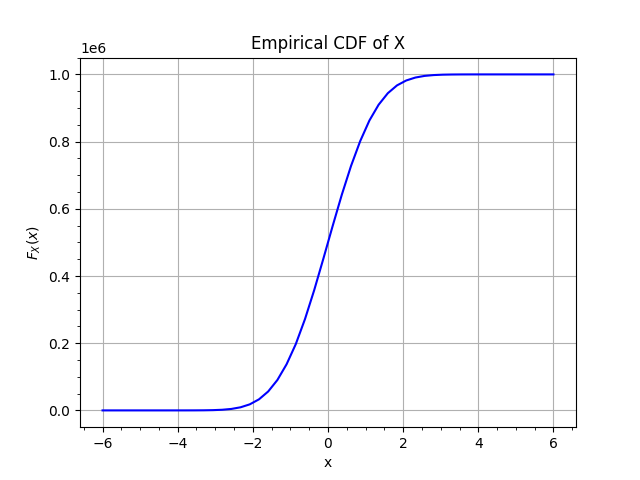
\includegraphics[width=\columnwidth]{./figs/fig2.2.png}
\caption{The CDF of $X$}
\label{fig:gauss_cdf}
\end{figure}
A CDF is a non-decreasing function. 
Its value varies from 0 to 1.
It is continuous if PDF has finite values.
%
\item
Load gau.dat in python and plot the empirical PDF of $X$ using the samples in gau.dat. The PDF of $X$ is defined as
\begin{align}
p_{X}\brak{x} = \frac{d}{dx}F_{X}\brak{x}
\label{eq:pdf_cdf}
\end{align}
What properties does the PDF have?
\\
\solution The empirical PDF of $X$ is plotted in Fig. \ref{fig:gauss_pdf} using the code below
\begin{lstlisting}
wget https://github.com/cs21btech11051Rajiv/AI1110_assignments/blob/main/manual1/q2/2p3.c
\end{lstlisting}
\begin{figure}[ht!]
\centering
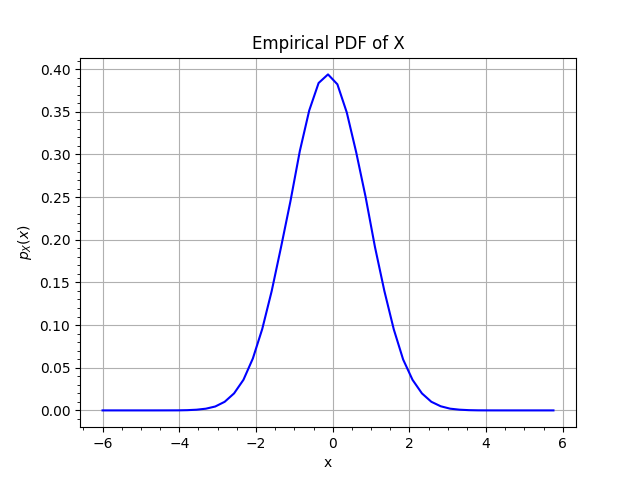
\includegraphics[width=\columnwidth]{./figs/fig2.3.png}
\caption{The PDF of $X$}
\label{fig:gauss_pdf}
\end{figure}
Values taken by a PDF are non negative. The total area under a PDF is equal to 1. 
%
\item Find the mean and variance of $X$ by writing a C program.
\\
\solution Run the following C file
\begin{lstlisting}
wget https://github.com/cs21btech11051Rajiv/AI1110_assignments/blob/main/manual1/q2/2p4.c
\end{lstlisting}
Results were, 
\begin{align}
E\sbrak{X}  = 0.000294 \\
\text{var}\sbrak{X}  = 0.999560
\end{align}
%
\item Given that 
\begin{align}
p_{X}\brak{x} = \frac{1}{\sqrt{2\pi}}\exp\brak{-\frac{x^2}{2}}, -\infty < x < \infty,
\end{align}
repeat the above exercise theoretically.
\\
\solution The theoretical PDF and CDF of $X$ is plotted in Fig. \ref{fig:theory_gauss_pdf} using the code below
\begin{lstlisting}
wget https://github.com/cs21btech11051Rajiv/AI1110_assignments/blob/main/manual1/q2/2p5.c
\end{lstlisting}
\begin{figure}[ht!]
    \centering
    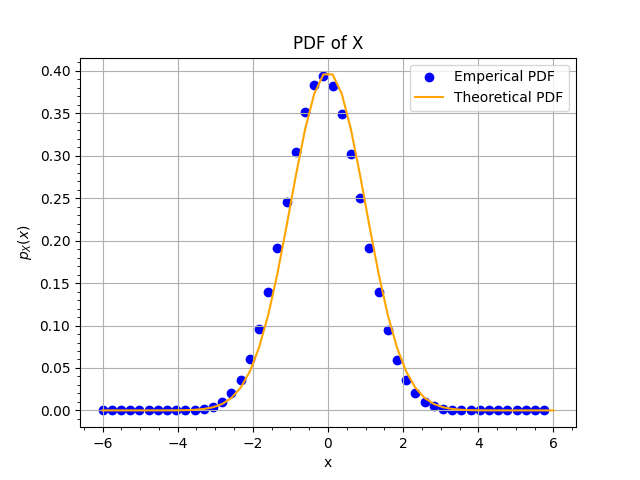
\includegraphics[width=\columnwidth]{./figs/fig2.5.png}
    \caption{The theoretical PDF of $X$}
    \label{fig:theory_gauss_pdf}
\end{figure}
\begin{figure}[ht!]
    \centering
    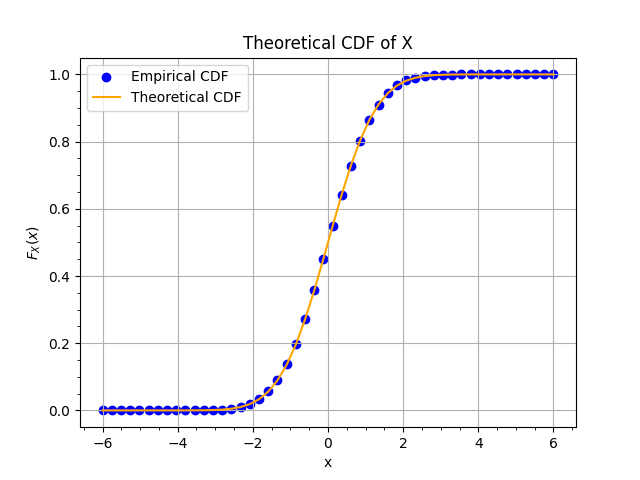
\includegraphics[width=\columnwidth]{./figs/fig2.5b.png}
    \caption{The theoretical CDF of $X$}
    \label{fig:theory_gauss_cdf}
\end{figure}
Using given equation \eqref{eq:expectation},
\begin{align}
    E\sbrak{X^k} &= \int_{-\infty}^{\infty}x^kdF_{X}\brak{x} \\
    E\sbrak{X} &= \int_{-\infty}^{\infty}x dF_{X}\brak{x} 
\end{align}
Using given equation \eqref{eq:pdf_cdf},
\begin{align}
    E\sbrak{X} &= \int_{-\infty}^{\infty}x p_{X}\brak{x} dx \\
    E\sbrak{X} &= \int_{-\infty}^{\infty}x
    \frac{1}{\sqrt{2\pi}}\exp\brak{-\frac{x^2}{2}} dx    
\end{align}
Taking $t = \frac{x^2}{2}$
\begin{align}
     E\sbrak{X} &= \int_{\infty}^{\infty}
    \frac{1}{\sqrt{2\pi}}\exp\brak{-\frac{t}{2}} dt \\
     E\sbrak{X} &= 0
\end{align}
To calculate variance we take k=2
\begin{align}
    \text{var}\sbrak{X} &= E\sbrak{\brak{X- E\sbrak{X}}^2} \\
    \text{var}\sbrak{X} &= E\sbrak{X^2} \\
    \text{var}\sbrak{X} &= \int_{-\infty}^{\infty}x^2dF_{X}\brak{x} \\
    \text{var}\sbrak{X} &= \int_{-\infty}^{\infty}x^2 p_{X}\brak{x} dx \\
    \text{var}\sbrak{X} &= \int_{-\infty}^{\infty}x^2
    \frac{1}{\sqrt{2\pi}}\exp\brak{-\frac{x^2}{2}} dx   
\end{align}
Integrating by parts, we obtain
\begin{multline}
    \text{var}\sbrak{X} = -x\frac{1}{\sqrt{2\pi}}\exp\brak{-\frac{x^2}{2}}  \Big|_{-\infty}^{\infty}  \\
    + \int_{-\infty}^{\infty}
    \frac{1}{\sqrt{2\pi}}\exp\brak{-\frac{x^2}{2}} dx   
\end{multline}
The second term is the area under the PDF, which is 1
\begin{align}
    \text{var}\sbrak{X} &= 0 + \int_{-\infty}^{\infty}p_{X}\brak{x}dx \\
    \text{var}\sbrak{X} &= 1   
\end{align}

%
\end{enumerate}
\section{From Uniform to Other}
\begin{enumerate}[label=\thesection.\arabic*
,ref=\thesection.\theenumi]
%
\item
Generate samples of 
%
\begin{align}
V = -2\ln\brak{1-U}
\end{align}
%
and plot its CDF.  
\\
\solution Run the following files to generate samples and CDF.
\begin{lstlisting}
wget https://github.com/cs21btech11051Rajiv/AI1110_assignments/blob/main/manual1/q3/3p1.c
wget https://github.com/cs21btech11051Rajiv/AI1110_assignments/blob/main/manual1/q3/3p1b.py
\end{lstlisting}
\begin{figure}[ht!]
\centering
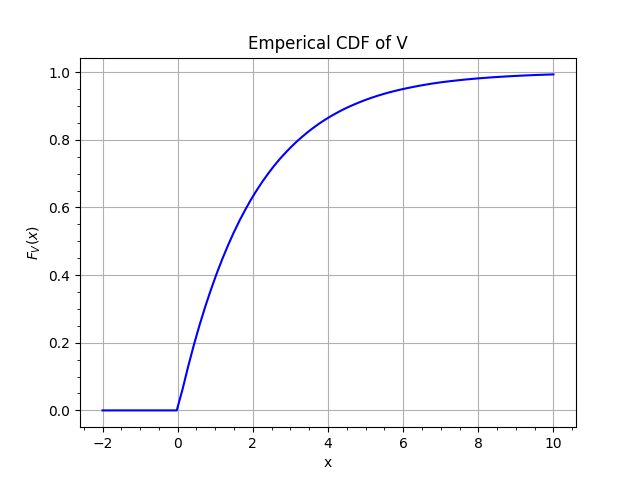
\includegraphics[width=\columnwidth]{./figs/fig3.1.png}
\caption{The CDF of $V$}
\label{fig:misc_cdf}
\end{figure}
\item Find a theoretical expression for $F_V\brak{x}$.
\\
\solution 
\begin{align}
	F_V\brak{x} &= Pr\brak{V\le x} \\
	F_V\brak{x} &= Pr\brak{-2\ln{\brak{1-U}} \le x}	\\
	F_V\brak{x} &= Pr\brak{\ln{\brak{1-U}} \ge -\frac{x}{2}}	\\
	F_V\brak{x} &= Pr\brak{1-U \ge \exp{\brak{-\frac{x}{2}} }}	\\
	F_V\brak{x} &= Pr\brak{U \le 1- \exp{\brak{-\frac{x}{2}} }} \\
	F_V\brak{x} &= F_U\brak{1- \exp{\brak{-\frac{x}{2}} }}		
\end{align}
\begin{small}
\begin{align}
	F_V\brak{x} &=
    \begin{cases}  
        0 & 1- \exp{\brak{-\frac{x}{2}} } < 0\\
        1- \exp{\brak{-\frac{x}{2}} } & 0 \le 1- \exp{\brak{-\frac{x}{2}} } \le 1 \\
        1 & 1 < 1- \exp{\brak{-\frac{x}{2}} }
    \end{cases}
\end{align}
\end{small}
This simplifies to
\begin{align}
	F_V\brak{x} &=
    \begin{cases}  
        0 & x < 0\\
        1- \exp{\brak{-\frac{x}{2}}} & x \ge 0
    \end{cases}
    \label{eq:F_V}
\end{align}
The following code plots the theoretical CDF.
\begin{lstlisting}
wget https://github.com/cs21btech11051Rajiv/AI1110_assignments/blob/main/manual1/q3/3p2.py
\end{lstlisting}
\begin{figure}[ht!]
\centering
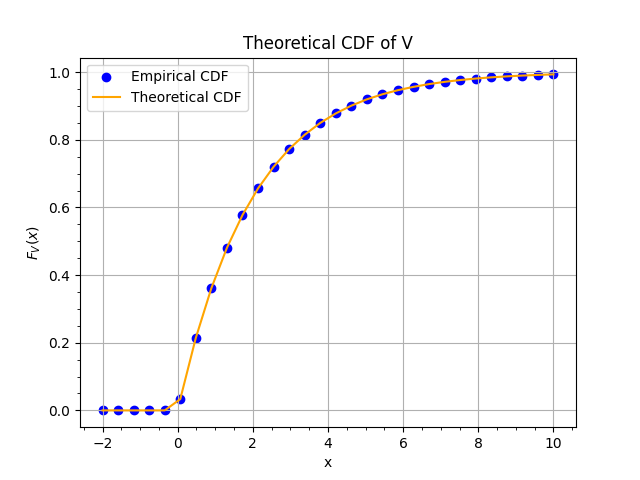
\includegraphics[width=\columnwidth]{./figs/fig3.2.png}
\caption{The CDF of $V$}
\label{fig:theory_misc_cdf}
\end{figure}

\end{enumerate}

\end{document}

